	\documentclass{article}
	\pagestyle{empty}
	\usepackage{amsmath} % Required for some math elements 
	\usepackage[utf8]{inputenc}
	
	\usepackage[usenames,dvipsnames,svgnames,table]{xcolor}
	\usepackage{tikz-timing}[2009/05/15]
	\usepackage{multicol}
	\usepackage[T2A]{fontenc}
	\usepackage[russian]{babel}
	\usepackage[left=2.5cm, right=1.5cm, vmargin=2.5cm]{geometry}
	\setlength\parindent{0pt} % Removes all indentation from paragraphs
	
	\usepackage{listings} %% собственно, это и есть пакет listing
	\usepackage{caption}
	\DeclareCaptionFont{white}{\color{white}} %% это сделает текст заголовка 
	\DeclareCaptionFormat{listing}{\colorbox{gray}{\parbox{\textwidth}{#1#2#3}}}
	\captionsetup[lstlisting]{format=listing,labelfont=white,textfont=white}
	\renewcommand\labelenumi{\theenumi)}	
	
	%\usepackage{times} % Uncomment to use the Times New Roman font
	
	%----------------------------------------------------------------------------------------
	%	DOCUMENT INFORMATION
	%----------------------------------------------------------------------------------------
	
	\begin{document}
	\lstset{ %
		language=c++,                 % выбор языка для подсветки (здесь это С)
		basicstyle=\small\sffamily, % размер и начертание шрифта для подсветки кода
		numbers=left,               % где поставить нумерацию строк (слева\справа)
		numberstyle=\tiny,           % размер шрифта для номеров строк
		stepnumber=1,                   % размер шага между двумя номерами строк
		firstnumber=1,
		numberfirstline=true
		numbersep=5pt,                % как далеко отстоят номера строк от подсвечиваемого кода
		backgroundcolor=\color{white}, % цвет фона подсветки - используем \usepackage{color}
		showspaces=false,            % показывать или нет пробелы специальными отступами
		showstringspaces=false,      % показывать или нет пробелы в строках
		showtabs=false,             % показывать или нет табуляцию в строках
		frame=single,              % рисовать рамку вокруг кода
		tabsize=2,                 % размер табуляции по умолчанию равен 2 пробелам
		captionpos=t,              % позиция заголовка вверху [t] или внизу [b] 
		breaklines=true,           % автоматически переносить строки (да\нет)
		breakatwhitespace=false, % переносить строки только если есть пробел
		escapeinside={\%*}{*)}   % если нужно добавить комментарии в коде
	}
	
	
	\begin{titlepage}
		
		
		\center % Center everything on the page
		
		%----------------------------------------------------------------------------------------
		%	HEADING SECTIONS
		%----------------------------------------------------------------------------------------
		
		ФЕДЕРАЛЬНОЕ ГОСУДАРСТВЕННОЕ АВТОНОМНОЕ ОБРАЗОВАТЕЛЬНОЕ УЧЕРЕЖДЕНИЕ ВЫСШЕГО ОБРАЗОВАНИЯ\linebreak  
		«Санкт-Петербургский политехнический университет Петра Великого»\\[2cm] % Name of your university/college
		\textsc{\Large Институт компьютерных наук и технологий}\\[6.5cm] % Major heading such as course name
		
		%----------------------------------------------------------------------------------------
		%	TITLE SECTION
		%----------------------------------------------------------------------------------------
		
		{ \huge \bfseries Курсовая работа	\\
			\Large \mdseries “Реализация Системы Массового Обслуживания”}\\[6.5cm] % Title of your document
		
		%----------------------------------------------------------------------------------------
		%	AUTHOR SECTION
		%----------------------------------------------------------------------------------------
		\begin{multicols}{2}
			\begin{flushright} \large
				
				{Выполнил студент группы: 33504/2:}\\[0.5cm]
				
				{Руководитель\\
					старший преподаватель}
				
			\end{flushright}
			\begin{flushright}
				
				{Лаппо С.С}\\[0.5cm] % Your nameГ
				
				
				Александрова О. В. % Supervisor's Name
				
			\end{flushright}
		\end{multicols}
		% If you don't want a supervisor, uncomment the two lines below and remove the section above
		%\Large \emph{Author:}\\
		%John \textsc{Smith}\\[3cm] % Your name
		
		%----------------------------------------------------------------------------------------
		%	DATE SECTION
		%----------------------------------------------------------------------------------------
		\flushright{
			{\today}\\[0.5cm] % Date, change the \today to a set date if you want to be precise
		}
		\centering{
			Санкт-Петербург\\
			2017
		}
		%----------------------------------------------------------------------------------------
		%	LOGO SECTION
		%----------------------------------------------------------------------------------------
		
		%\includegraphics{Logo}\\[1cm] % Include a department/university logo - this will require the graphicx package
		
		%----------------------------------------------------------------------------------------
		
		\vfill % Fill the rest of the page with whitespace
		
	\end{titlepage}
	
	% Содержание
	
	\tableofcontents
	\newpage
	
	% If you wish to include an abstract, uncomment the lines below
	% \begin{abstract}
	% Abstract text
	% \end{abstract}
	
	%----------------------------------------------------------------------------------------
	%	SECTION 1
	%----------------------------------------------------------------------------------------
	
	\section{Постановка задачи}
	Целью курсовой работы является создание модели вычислительной системы (ВС) или ее части на некотором уровне детализации, описывающей и имитирующей ее структуру и функциональность.\\
	Каждый реальный объект (реальная ВС) обладает бесконечной сложностью, множеством характеристик, внутренних и внешних связей. Модель есть приближенное описание объекта с целью получения требуемых результатов с определенной точностью и достоверностью.\\
	При необходимости исследования поведенческих характеристик ВС в процессе исследования выгодно использовать не сам объект, а его модель. Степень приближения модели к описываемому объекту может быть различной и зависит от требований задачи.\\
	Существуют различные типы моделей:
	\begin{enumerate}
		\item Аналитические (математические) модели
		\item Аналоговые модели
		\item Физические модели
		\item Имитационные модели 
	\end{enumerate}
	Последний тип моделей является предметом нашего изучения. Одним из подходов к построению имитационной модели является построение ее в виде системы массового обслуживания (СМО), с характерной для СМО терминологией: источник, буфер, прибор, диспетчер, заявка (требование).
	Существуют два подхода к построению моделирующего алгоритма:
	\subsection{Принцип $\Delta$t}
	Принцип $\Delta$t
	Универсальный метод построения моделирующего алгоритма, когда
	состояние объекта проверяется через фиксированный интервал
	модельного времени. Суть его заключается в следующем: в каждый
	момент времени t получают приближенные значения характеристик исследуемого объекта.  $\Delta$t можно получить детерминированным способом.
	Основной критерий выбора  $\Delta$t — он должен быть настолько мал, чтобы не пропустить событие в моделируемой системе, которое должно быть учтено при выбранной детальности моделирования. Метод неэффективен, т.к. постоянно проверяет состояние объектов моделирования, не изменяющихся при этом, особенно при малых  $\Delta$t.
	
	
	\subsection{Принцип особых состояний}
	При исследовании реальной системы интервалы, в которых состояние ее не меняется, не представляют интереса. Имеют значение только переходы системы из одного состояния в другое в некоторые моменты времени. Эти переходы определяются особыми состояниями или событиями.\\
	Рассмотрим некоторые типы особых событий, которые изменяют состояние системы:
	\begin{enumerate}
		\item Поступление заявки в СМО (момент генерации заявки источником);
		\item Освобождение прибора (готовность прибора взять заявку на обслуживание);
		\item Окончание процесса моделирования.
	\end{enumerate}
	Использование принципа особых событий для построения имитационной модели наиболее эффективно. В настоящей курсовой работе предлагается использовать именно этом принцип.
	
	\newpage
	%----------------------------------------------------------------------------------------
	%	SECTION 2
	%----------------------------------------------------------------------------------------
	\section{Формализованная схема и описание СМО.}
	
	\begin{figure}[!htbp]
	\centering
	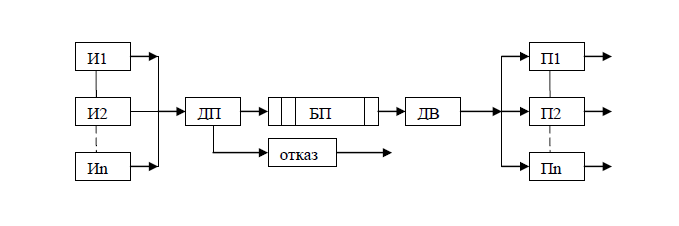
\includegraphics[width=\textwidth,height=\textheight,keepaspectratio]{smo.png}\\
	\caption{Формализованная схема СМО}	
	\end{figure}
	Здесь Иi (i= 1..n) – источник заявок, который генерирует заявки, а
	все вместе n источников создают входной поток заявок в систему.
	Каждая заявка приходит в СМО со своими характеристиками.
	Это входное T — время генерации заявки (время поступления её в СМО) и номер заявки составленный из номера источника, сгенерировавшего заявку, и порядкового номера заявки от этого источника. Например, (2.3) – третья заявка от второго источника.\\
	П — приборы, которые обслуживают заявки и создают выходной
	поток заявок после обслуживания.\\
	БП — буферная память (место для хранения очереди заявок).
	В общей памяти хранятся заявки от различных источников.
	Порядок их записи в БП определяется только дисциплиной
	буферизации.\\
	ДП — диспетчер постановки заявок.\\
	ДВ — диспетчер выбора заявок.\\
	\subsection{Вариант рассматриваемой мной СМО}
	ИБ	ИЗ1	ПЗ2	Д10З1	Д10О3	Д2П1	Д2Б3	ОР1	ОД3\\
	Источники:\\
	ИБ – бесконечный источник;\\
	И31 – Пуассоновский закон распределения заявок;\\
	Приборы:\\
	П32 – равномерный закон распределения времени обслуживания;\\
	Описание дисциплин постановки и выбора:\\
	Дисциплина буферизации:\\	
	Д1031 – по кольцу;\\
	Дисциплина отказа:\\
	Д1003 – самая старая заявка в буфере; \\
	Д2П1 – приоритет прибора по номеру;\\
	Д2Б3 – выбор из буфера по кольцу;\\
	Динамическое отражение результатов:\\
	ОД3 – сводная таблица результатов;\\
	Отражение результатов после сбора статистики:\\
	ОР1 – текущее состояние.\\
	
	\section{Временная диаграмма функционирования системы}
	Исходя из заданного задания на работу рассмотрим, как должна будет функционировать система массового обслуживания на временной диаграмме. Для примера возьмем 3 источника (И1, И2, И3), 4 позиции в буфере (Б1, Б2, Б3, Б4) и 5 приборов (П1, П2, П3, П4, П5). В результате получим следующую диаграмму: 
	\begin{tikztimingtable}
		И1 				& L G L L L L L L G L L L L G L L L L L L L L G L L L L G L L L L L L L L G L\\
		И2 				& L L L G L L L L L L L L L L G L L L L L L L L L L L L G L L L L G L L L\\
		И3 				& L L L L L G L L L L G L L L L L L L L L L L L G L L L L L L G L L L L L\\
		П1 				& L 3D{1} L L L 4D{1} L L 3D{2} L L L 7D{1} L 5D{3}\\
		П2 				& L L L 4D{2} L L 2D{3} L L L L L L L L L L 11D{3}\\
		П3 				& L L L L L 5D{3} L L L L L L L L L L L L L L L L 6D{2}\\
		П4 				& L L L L L L L L L L L L L L L L L L L L L L L L L L L L L 3D{2}\\
		П5 				& L L L L L L L L L L L L L L L L L L L L L L L L L L L L L L L D{1}\\
		Б1 				& L G L L L L L L L L L L L L G L L L L L L L L L L L L L L L L G L L L\\
		Б2 				& L L L G L L L L L L L L L L L L L L L L G L L L L L L L L L L L L G L\\
		Б3 				& L L L L L G L L L L L L L L L L L L L L L L G L L L L L L L L L L L\\
		Б4 				& L L L L L L L G L L L L L L L L L L L L L L L L L L G L L L L L L L\\
		Б5 				& L L L L L L L L L G L L L L L L L L L L L L L L L L L L G L L L L L\\
		\\
		Постановка      & L G L L G L L G L L G L L G L L L L G L L L L L L G L L G L L L L G L L G L L G L L G L\\
		Изъятие         & L G L L G L L G L L G L L G L L L L G L L L L L L G L L G L L L L G L L G L L G L L G L\\
		\extracode
		\tablerules
		\begin{pgfonlayer}{background}
		\end{pgfonlayer}
	\end{tikztimingtable}
	\newpage
	\section{Вывод законов распределения}
	\subsection{Пуассоновский закон распределения }
	\begin{equation*}F_k=\frac{e^{-\gamma}*\gamma^k}{k!}
	\end{equation*}
	Где $\gamma$ - заданное значение.\\
	
	\begin{equation*}x=\frac{-1}{\gamma}*\ln(F_k)\end{equation*}
	В программе данное выражение записано следующим образом:\\
	\lstinline|this->last_time_of_gen += (-1/lambda)*log((double)qrand()/RAND_MAX);|
	
	\subsection{Равномерный закон распределения}
	\begin{equation*}
	F(x)=
	\begin{cases}
	0<, x<a, 
	\\
	\frac{x-a}{x-b}, a \le x \le b,
	\\
	1, x\ge b.
	\end{cases}
	\end{equation*}
	где a и b – заданные значения. 
	\begin{equation*}
	x=F(x)(b-a)+a
	\end{equation*}
	В программе данное выражение записано следующим образом:\\
	\lstinline|double rand_time=(double)a+(double)(b-a)*(rand()%100)/100;|
	\newpage
	\section{Пример технической системы (ВС или части ВС), удовлетворяющей формализованному описанию}
	\centering
	\begin{tabular}{|p{5.2cm}|p{12cm}|}
		\hline
		Техническая система & Автомобильный парктроник\\ \hline
		Источники & Источниками являются датчики расстояния, которые отсылают данные на обработку в виде пакета размером 64 Кбайт. Необходимо получать и обрабатывать информацию с максимального датчиков. \\ \hline		
		Приборы	&Приборами являются ЭВМ, которые обрабатывают полученную информацию и отправляют результирующий сигнал на дисплей. \\ \hline	
		Буфер & Буфером является буфер коммутатора, который может быть от 64 Кбайт (1 заявка) и может быть наращен до 256 кб (4 заявки) с шагом 64 Кбайт. \\ \hline		
		Дисциплина постановки в буфер & Постановка по кольцу\\ \hline
		Дисциплина выборки из буфера & Выборка по кольцу. Мы разом получаем всю информацию о необходимых изменениях в расположении автомобиля и в порядке приоритетности отправляем заявки на обработку.\\ \hline
		Дисциплина отказа & Самая старая заявка в буфере\\ \hline
		Дисциплина постановки на обслуживание & Приоритет по номеру прибора\\ \hline
		
	\end{tabular} \\
	\flushleft
	\section{Ограничения и требуемые характеристики:}
	Вероятность отказа должна составлять не более 10\%.\\
	Загрузка приборов более 90\%.\\
	Время пребывания заявки в системе не более 10 мс.
	Рассматриваемый диапазон характеристик системы и доступные типы процессоров и характеристики программного-аппаратного комплекса, построенного на данном типе процессора приведены ниже в таблицах компонентов системы.\\
	\centering
	\begin{tabular}{|p{5.2cm}|p{6.5cm}|}
		\hline
		Количество датчиков расстояния    & От 2 до 6                            \\ \hline
		Вес заявки                & 64 Кб                                \\ \hline
		Объем буфера              & От 64Кб до 256 Кб                    \\ \hline
		Количество приборов       & От 1 до 7                            \\ \hline
		Скорость генерации заявок & Пуассоновский поток с $\lambda = 3$ мс. \\ \hline
		Скорость обработки заявок & Равномерный поток с границами(мс):   \\
		~                         & 1. [4;5]                             \\
		~                         & 2. [5;6]                             \\
		~                         & 3. [6;7]                             \\ \hline
	\end{tabular}
	\flushleft
	Стоимость компонентов системы:\\
	Считаем, что количество датчиков строго сконфигурировано: 2/3 спереди и сзади  автомобиля, поэтому стоимость их не учитывается. Нужно подобрать минимальную конфигурацию по размеру буфера и количеству приборов, удовлетворяющих условиям, для наименьших затрат, связанных с их покупкой. Условимся, что стоимость одного прибора для обработки со временем обслуживания:\\
	\begin{enumerate}
	\item От 3 до 4 мс – 25000 рублей;
	\item От 5 до 6 мс – 12000 рублей;
	\item От 6 до 7 мс – 8000 рублей.
	\end{enumerate}
	Стоимость расширения буфера на 1 слот – 3000 рублей.
	\newpage
	\section{Документация на ПО}
	\subsection{Блок-схема}
	Приведем для понимания работы программы обобщенную блок-схему:
	\begin{figure}[!htbp]
	\centering
	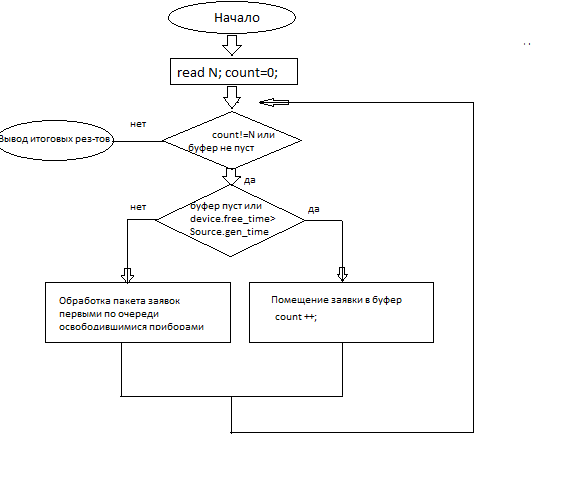
\includegraphics[width=\textwidth,height=\textheight,keepaspectratio]{smo1.png}\\
	\caption{Описание работы программы}
	\end{figure}
	\subsection{Модульная структура}
	Разработка производилась в среде Qt creator на языке C++ с использованием графической библиотеки Qt.\\
	Приложение использует объектно-ориентированную парадигму программирования и содержит набор классов:\\
	\begin{enumerate}
	\item BufferQueue - класс буфера;
	\item mainwindow - класс ui, создающий весь интерфейс;
	\item OperatingDevice - класс прибора;
	\item SourceDevice - класс источника;
	\item StatisticsController - класс, отвечающий за обработку статистики;
	\item SystemController - класс, который занимается управлением системой;
	\item SystemEvent - класс, характеризующий системные события;
	\item SystemTask - класс, характерищующий задачу.
	\end{enumerate}
	Программа содержит точку входа в файле main.cpp. Основное действие процедуры main – создание объекта окна программы и его отображение. После появления окна программы, запускается цикл обработки событий (действий пользователя).
	Отображение результатов в автоматическом режиме:\\
	\begin{figure}[!htbp]
		\centering
		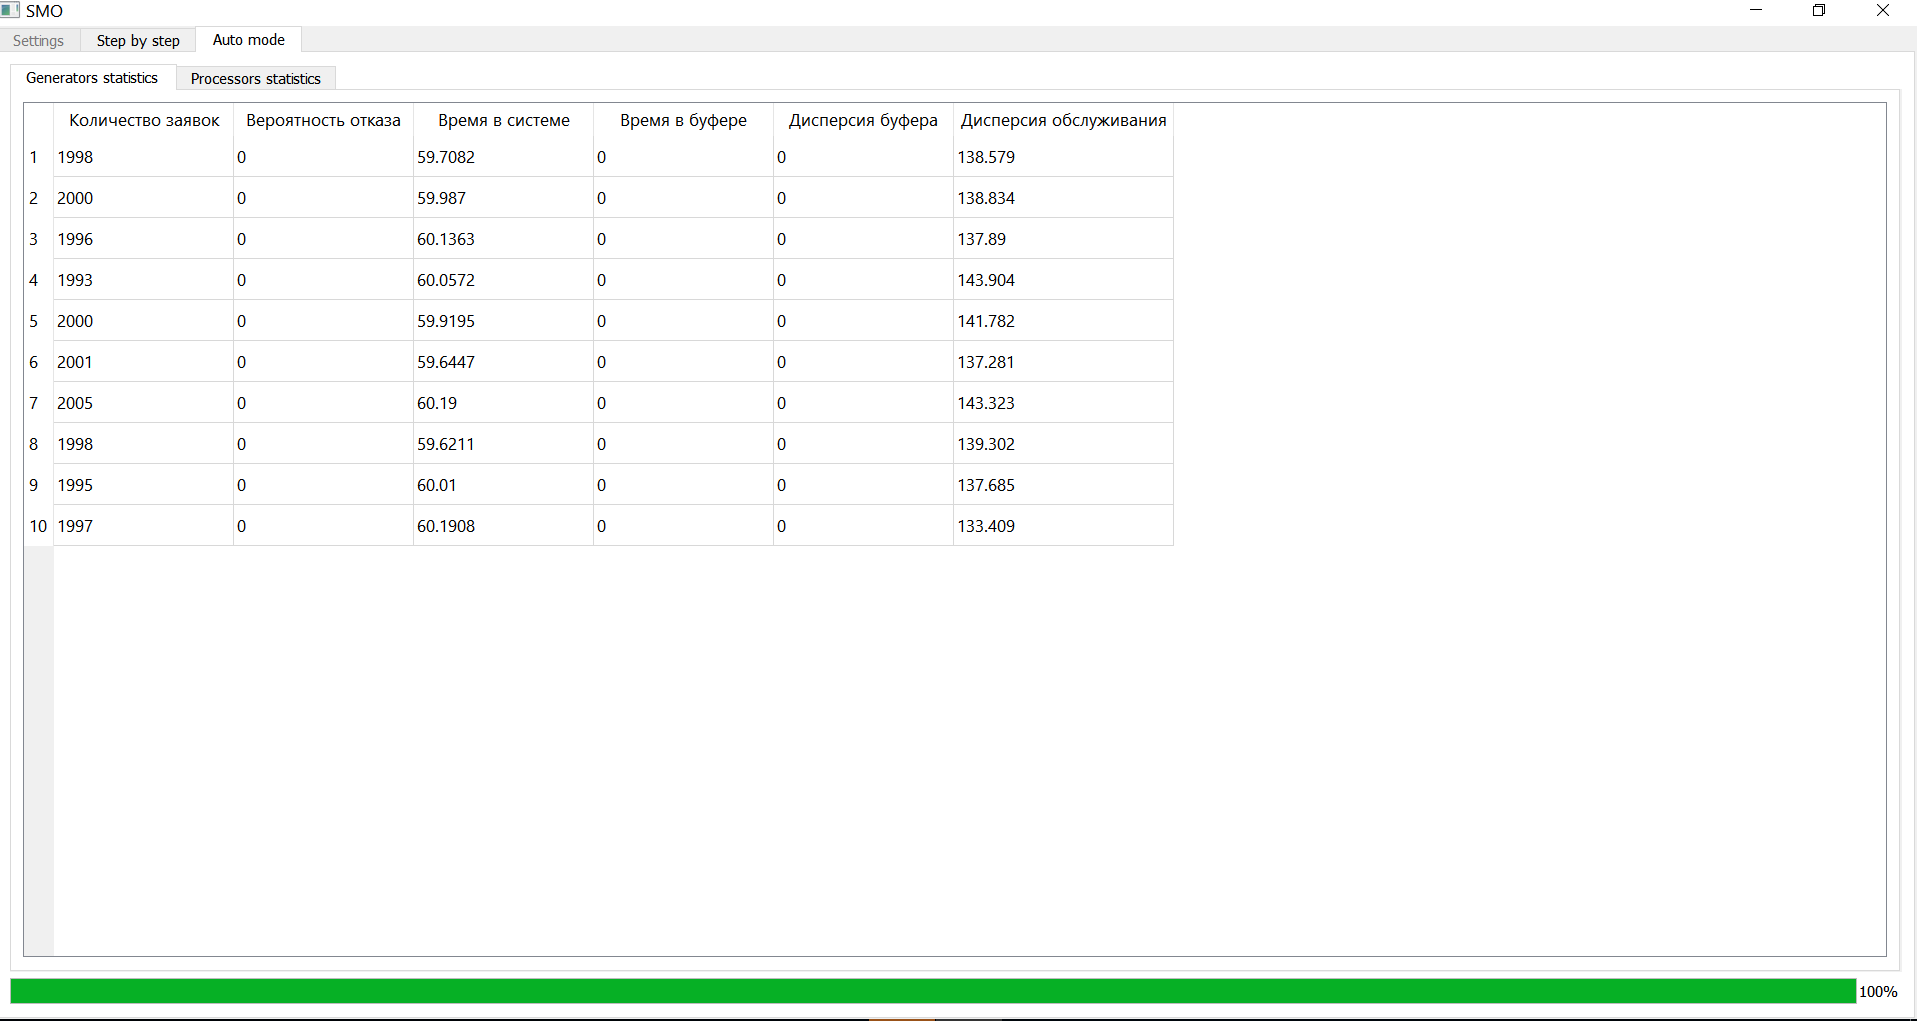
\includegraphics[width=\textwidth,height=200pt,keepaspectratio]{auto_1.png}\\
		\caption{Отображение статистики источников}
	\end{figure}
	\begin{figure}[!htbp]
		\centering
		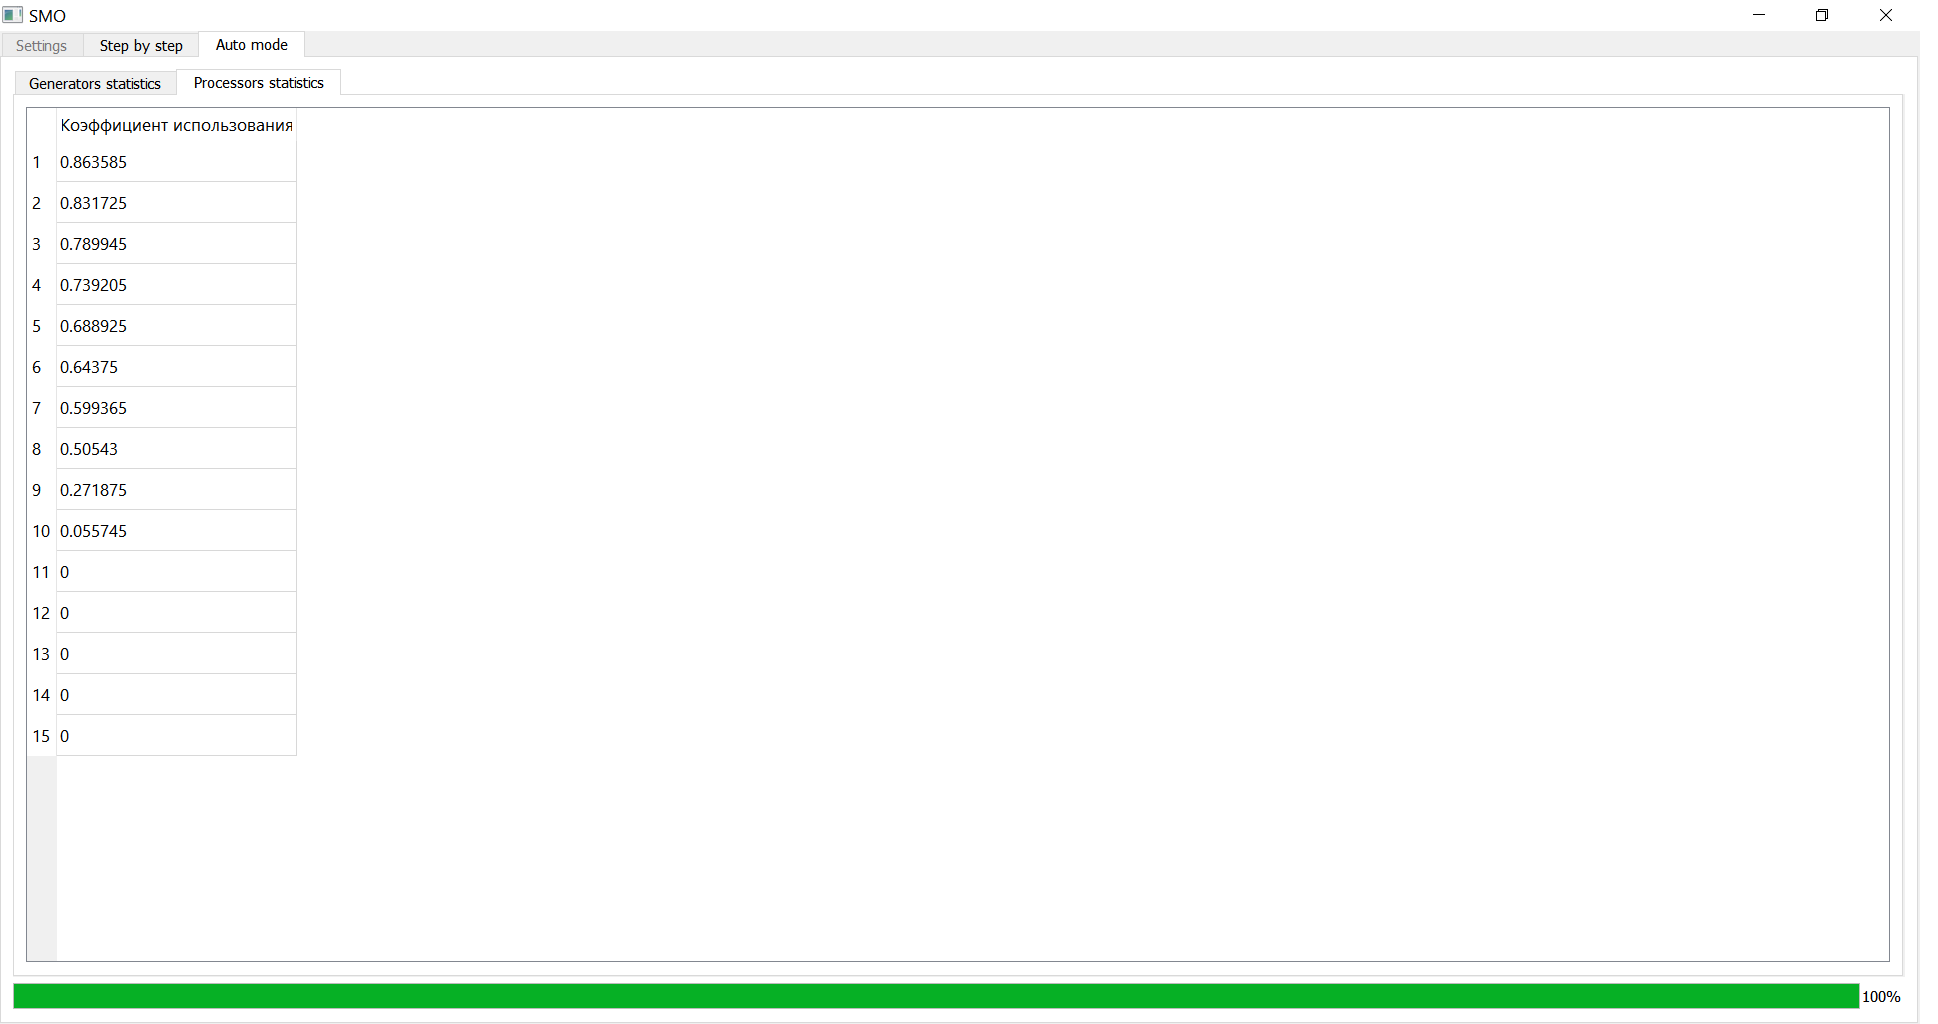
\includegraphics[width=\textwidth,height=200pt,keepaspectratio]{auto_2.png}\\
		\caption{Отображение статистики приборов}
	\end{figure}
	\newpage
	Отображение результатов в пошаговом режиме:	
	\begin{figure}[!htbp]
		\centering
		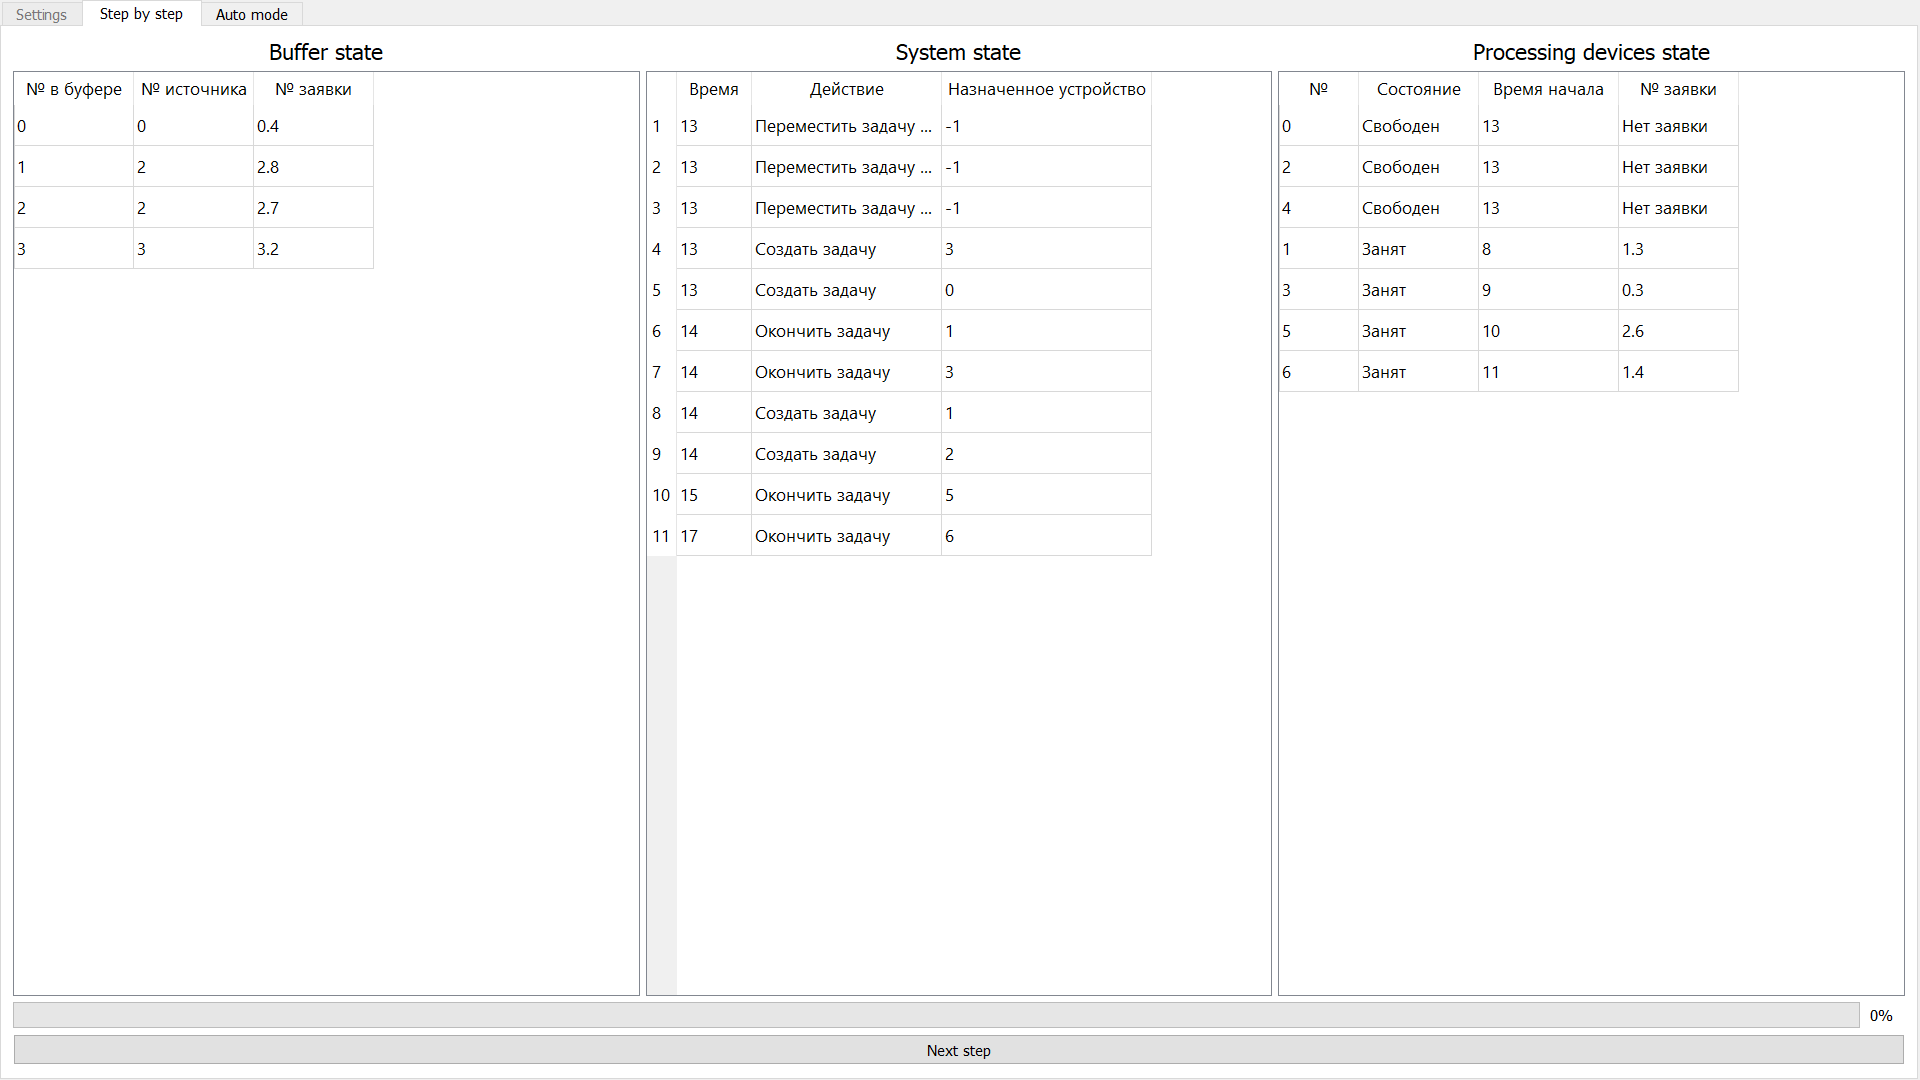
\includegraphics[width=\textwidth,height=250pt,keepaspectratio]{man_1.png}\\
		\caption{Пошаговый режим}
	\end{figure}
	\clearpage
	\section{Результаты работы имитационной модели}
	\subsection{Определение количества реализаций}
	\flushleft
	Количество реализаций, необходимое для получения нужной точности при заданной доверительной вероятности, можно оценивать
	по формуле:
	\begin{equation*}
		N=\frac{t^2_\alpha(1-p)}{p\delta^2}
	\end{equation*}
	где p — вероятность отказа заявкам в обслуживании,\\
	$t_\alpha=1.643$, для $\alpha = 0.9$,\\
	$\sigma=0.1$ - относительная точность.
	По результатам работы программы получено, что в большинстве
	случаев для достижения заданной точности необходимо от 3000 до
	5000 заявок. Однако, в случаях, когда p мало (<0.05) для достижения
	точности в 10\% может потребоваться существенно больше заявок
	(20000-30000).
	\subsection{Анализ результатов, выводы и рекомендации по выбору конфигурации системы.}
	Рассмотрим первый возможный вариант конфигурации, когда имеется по два источника спереди и сзади.
	Т.к. целью моделирования является выбор конфигурации
	системы, требующей наименьшее количество ресурсов и
	обрабатывающей максимальный поток информации, то начнем с проверки конфигурации с минимальным числом приборов и мин. размером буфера.\\
	Количество источников во всех опытах возьмем равным 4.
	\begin{tabular}{|p{2.1cm}|p{2.1cm}|p{0.5cm}|p{2.1cm}|p{2.1cm}|p{2.1cm}|p{2.1cm}|p{2.1cm}|}
		\hline
		Число источников&Число приборов&a;b&lambda&Размер буфера&Вероятность отказа&Т преб&Коэф. использ.\\ \hline
		4&1&6;7&3&1&0,87&1,5&1\\ \hline
	\end{tabular}
	В первом опыте прибор эффективно используется, время нахождения в системе допустимо, но 87\% заявок уходят в отказ, что является недопустимым, поэтому расширяем буфер.
	\begin{tabular}{|p{2.1cm}|p{2.1cm}|p{0.5cm}|p{2.1cm}|p{2.1cm}|p{2.1cm}|p{2.1cm}|p{2.1cm}|}
		\hline
		Число источников&Число приборов&a;b&lambda&Размер буфера&Вероятность отказа&Т преб&Коэф. использ.\\ \hline
		4&1&6;7&3&4&0,87&2,96&0,999\\ \hline
	\end{tabular}
	Вероятность отказа не снизилась, и до сих пор не является удовлетворительной. Время нахождения в системе допустимо. Возьмем для обработки 3 самых дешевых прибора.
	\begin{tabular}{|p{2.1cm}|p{2.1cm}|p{0.5cm}|p{2.1cm}|p{2.1cm}|p{2.1cm}|p{2.1cm}|p{2.1cm}|}
		\hline
		Число источников&Число приборов&a;b&lambda&Размер буфера&Вероятность отказа&Т преб&Коэф. использ.\\ \hline
		4&3&6;7&3&4&0,66&2,87&0,999\\ \hline
	\end{tabular}
	Увеличим количество приборов до 7(максимум) самых дешевых
	\begin{tabular}{|p{2.1cm}|p{2.1cm}|p{0.5cm}|p{2.1cm}|p{2.1cm}|p{2.1cm}|p{2.1cm}|p{2.1cm}|}
		\hline
		Число источников&Число приборов&a;b&lambda&Размер буфера&Вероятность отказа&Т преб&Коэф. использ.\\ \hline
		4&7&6;7&3&4&0,2&7,42&0,995\\ \hline
	\end{tabular}
	Время нахождения в системе допустимо. Вероятность отказа упала, но все еще достаточно велика, поэтому возьмем приборы со средними характеристиками
	\begin{tabular}{|p{2.1cm}|p{2.1cm}|p{0.5cm}|p{2.1cm}|p{2.1cm}|p{2.1cm}|p{2.1cm}|p{2.1cm}|}
		\hline
		Число источников&Число приборов&a;b&lambda&Размер буфера&Вероятность отказа&Т преб&Коэф. использ.\\ \hline
		4&7&5;6&3&4&0,06&6,54&0,94\\ \hline
	\end{tabular}
	Время нахождения в системе допустимо. Вероятность отказа снизилась до 6\%, что нас полностью устраивает. При уменьшении количества приборов (и даже при улучшении их качества) система либо не будет удовлетворять требованиям, либо обойдется нам дороже.\\
	Стоимость системы (без учета цен на датчики): 12000*7+3000*4=96000 рублей.\\
	Теперь рассмотрим систему, когда количество датчиков на торцах автомобиля увеличено до 3.\\
	Попробуем вначале использовать аналогичную предыдщему случаю конфигурацию:
	\begin{tabular}{|p{2.1cm}|p{2.1cm}|p{0.5cm}|p{2.1cm}|p{2.1cm}|p{2.1cm}|p{2.1cm}|p{2.1cm}|}
		\hline
		Число источников&Число приборов&a;b&lambda&Размер буфера&Вероятность отказа&Т преб&Коэф. использ.\\ \hline
		6&7&5;6&3&4&0,36&5,19&0,99\\ \hline
	\end{tabular}
	Время обработки недопустимо. Возьмём самые лучшие приборы.
	\begin{tabular}{|p{2.1cm}|p{2.1cm}|p{0.5cm}|p{2.1cm}|p{2.1cm}|p{2.1cm}|p{2.1cm}|p{2.1cm}|}
		\hline
		Число источников&Число приборов&a;b&lambda&Размер буфера&Вероятность отказа&Т преб&Коэф. использ.\\ \hline
		6&7&3;4&3&4&0,04&4.11&0,88\\ \hline
	\end{tabular}
	При данной конфигурации количество отказов минимально, также значительно сократилось время нахождения в системе. Попробуем уменьшить количество приборов.
	\begin{tabular}{|p{2.1cm}|p{2.1cm}|p{0.5cm}|p{2.1cm}|p{2.1cm}|p{2.1cm}|p{2.1cm}|p{2.1cm}|}
		\hline
		Число источников&Число приборов&a;b&lambda&Размер буфера&Вероятность отказа&Т преб&Коэф. использ.\\ \hline
		6&6&3;4&3&4&0,14&4.37&0,98\\ \hline
	\end{tabular}
	Время нахождения в системе осталось в допустимых пределах, загрузка приборов более оптимальна, однако мы незначительно превысили порог отказов, так что этот вариант нам недоступен.\\
	Попробуем альтернативное удешевление системы - уменьшим количество мест в буфере.
	
	\begin{tabular}{|p{2.1cm}|p{2.1cm}|p{0.5cm}|p{2.1cm}|p{2.1cm}|p{2.1cm}|p{2.1cm}|p{2.1cm}|}
		\hline
		Число источников&Число приборов&a;b&lambda&Размер буфера&Вероятность отказа&Т преб&Коэф. использ.\\ \hline
		6&7&3;4&3&2&0,07&3.56&0,90\\ \hline
	\end{tabular}
	Дальнейшее уменьшение буфера приведёт к превышению допустимого времени обработки, а данная конфигурация нас полностью устраивает.
	
	Стоимость системы (без учета цен на датчики): 25000*7+3000*2=181000 рублей.\\
	\newpage
	\section{Выводы}
	В ходе выполнения курсовой работы мной была написана система массового обслуживания на языке C++ в среде разработки Qt Creator с использованием библиотеки Qt. С помощью получившейся программы была проанализирована реальная система и подобрана максимально выгодная комплектация данной системы.
	%----------------------------------------------------------------------------------------
	%	BIBLIOGRAPHY
	%----------------------------------------------------------------------------------------
	
	%\bibliographystyle{apalike}
	
	%\bibliography{sample}
	
	%----------------------------------------------------------------------------------------
	
	
	\end{document}